\documentclass[12,]{article}
\usepackage{lmodern}
\usepackage{amssymb,amsmath}
\usepackage{ifxetex,ifluatex}
\usepackage{fixltx2e} % provides \textsubscript
\ifnum 0\ifxetex 1\fi\ifluatex 1\fi=0 % if pdftex
  \usepackage[T1]{fontenc}
  \usepackage[utf8]{inputenc}
\else % if luatex or xelatex
  \ifxetex
    \usepackage{mathspec}
  \else
    \usepackage{fontspec}
  \fi
  \defaultfontfeatures{Ligatures=TeX,Scale=MatchLowercase}
\fi
% use upquote if available, for straight quotes in verbatim environments
\IfFileExists{upquote.sty}{\usepackage{upquote}}{}
% use microtype if available
\IfFileExists{microtype.sty}{%
\usepackage{microtype}
\UseMicrotypeSet[protrusion]{basicmath} % disable protrusion for tt fonts
}{}
\usepackage[margin=1in]{geometry}
\usepackage{hyperref}
\hypersetup{unicode=true,
            pdftitle={Programmieren mit R: Seminararbeit\_1},
            pdfauthor={Daniyar Akhmetov (5127348); Marcelo Rainho Avila (4679876); Xuan Son Le (4669361)},
            pdfborder={0 0 0},
            breaklinks=true}
\urlstyle{same}  % don't use monospace font for urls
\usepackage{color}
\usepackage{fancyvrb}
\newcommand{\VerbBar}{|}
\newcommand{\VERB}{\Verb[commandchars=\\\{\}]}
\DefineVerbatimEnvironment{Highlighting}{Verbatim}{commandchars=\\\{\}}
% Add ',fontsize=\small' for more characters per line
\usepackage{framed}
\definecolor{shadecolor}{RGB}{248,248,248}
\newenvironment{Shaded}{\begin{snugshade}}{\end{snugshade}}
\newcommand{\KeywordTok}[1]{\textcolor[rgb]{0.13,0.29,0.53}{\textbf{#1}}}
\newcommand{\DataTypeTok}[1]{\textcolor[rgb]{0.13,0.29,0.53}{#1}}
\newcommand{\DecValTok}[1]{\textcolor[rgb]{0.00,0.00,0.81}{#1}}
\newcommand{\BaseNTok}[1]{\textcolor[rgb]{0.00,0.00,0.81}{#1}}
\newcommand{\FloatTok}[1]{\textcolor[rgb]{0.00,0.00,0.81}{#1}}
\newcommand{\ConstantTok}[1]{\textcolor[rgb]{0.00,0.00,0.00}{#1}}
\newcommand{\CharTok}[1]{\textcolor[rgb]{0.31,0.60,0.02}{#1}}
\newcommand{\SpecialCharTok}[1]{\textcolor[rgb]{0.00,0.00,0.00}{#1}}
\newcommand{\StringTok}[1]{\textcolor[rgb]{0.31,0.60,0.02}{#1}}
\newcommand{\VerbatimStringTok}[1]{\textcolor[rgb]{0.31,0.60,0.02}{#1}}
\newcommand{\SpecialStringTok}[1]{\textcolor[rgb]{0.31,0.60,0.02}{#1}}
\newcommand{\ImportTok}[1]{#1}
\newcommand{\CommentTok}[1]{\textcolor[rgb]{0.56,0.35,0.01}{\textit{#1}}}
\newcommand{\DocumentationTok}[1]{\textcolor[rgb]{0.56,0.35,0.01}{\textbf{\textit{#1}}}}
\newcommand{\AnnotationTok}[1]{\textcolor[rgb]{0.56,0.35,0.01}{\textbf{\textit{#1}}}}
\newcommand{\CommentVarTok}[1]{\textcolor[rgb]{0.56,0.35,0.01}{\textbf{\textit{#1}}}}
\newcommand{\OtherTok}[1]{\textcolor[rgb]{0.56,0.35,0.01}{#1}}
\newcommand{\FunctionTok}[1]{\textcolor[rgb]{0.00,0.00,0.00}{#1}}
\newcommand{\VariableTok}[1]{\textcolor[rgb]{0.00,0.00,0.00}{#1}}
\newcommand{\ControlFlowTok}[1]{\textcolor[rgb]{0.13,0.29,0.53}{\textbf{#1}}}
\newcommand{\OperatorTok}[1]{\textcolor[rgb]{0.81,0.36,0.00}{\textbf{#1}}}
\newcommand{\BuiltInTok}[1]{#1}
\newcommand{\ExtensionTok}[1]{#1}
\newcommand{\PreprocessorTok}[1]{\textcolor[rgb]{0.56,0.35,0.01}{\textit{#1}}}
\newcommand{\AttributeTok}[1]{\textcolor[rgb]{0.77,0.63,0.00}{#1}}
\newcommand{\RegionMarkerTok}[1]{#1}
\newcommand{\InformationTok}[1]{\textcolor[rgb]{0.56,0.35,0.01}{\textbf{\textit{#1}}}}
\newcommand{\WarningTok}[1]{\textcolor[rgb]{0.56,0.35,0.01}{\textbf{\textit{#1}}}}
\newcommand{\AlertTok}[1]{\textcolor[rgb]{0.94,0.16,0.16}{#1}}
\newcommand{\ErrorTok}[1]{\textcolor[rgb]{0.64,0.00,0.00}{\textbf{#1}}}
\newcommand{\NormalTok}[1]{#1}
\usepackage{longtable,booktabs}
\usepackage{graphicx,grffile}
\makeatletter
\def\maxwidth{\ifdim\Gin@nat@width>\linewidth\linewidth\else\Gin@nat@width\fi}
\def\maxheight{\ifdim\Gin@nat@height>\textheight\textheight\else\Gin@nat@height\fi}
\makeatother
% Scale images if necessary, so that they will not overflow the page
% margins by default, and it is still possible to overwrite the defaults
% using explicit options in \includegraphics[width, height, ...]{}
\setkeys{Gin}{width=\maxwidth,height=\maxheight,keepaspectratio}
\IfFileExists{parskip.sty}{%
\usepackage{parskip}
}{% else
\setlength{\parindent}{0pt}
\setlength{\parskip}{6pt plus 2pt minus 1pt}
}
\setlength{\emergencystretch}{3em}  % prevent overfull lines
\providecommand{\tightlist}{%
  \setlength{\itemsep}{0pt}\setlength{\parskip}{0pt}}
\setcounter{secnumdepth}{5}
% Redefines (sub)paragraphs to behave more like sections
\ifx\paragraph\undefined\else
\let\oldparagraph\paragraph
\renewcommand{\paragraph}[1]{\oldparagraph{#1}\mbox{}}
\fi
\ifx\subparagraph\undefined\else
\let\oldsubparagraph\subparagraph
\renewcommand{\subparagraph}[1]{\oldsubparagraph{#1}\mbox{}}
\fi

%%% Use protect on footnotes to avoid problems with footnotes in titles
\let\rmarkdownfootnote\footnote%
\def\footnote{\protect\rmarkdownfootnote}

%%% Change title format to be more compact
\usepackage{titling}

% Create subtitle command for use in maketitle
\newcommand{\subtitle}[1]{
  \posttitle{
    \begin{center}\large#1\end{center}
    }
}

\setlength{\droptitle}{-2em}
  \title{Programmieren mit R: Seminararbeit\_1}
  \pretitle{\vspace{\droptitle}\centering\huge}
  \posttitle{\par}
  \author{Daniyar Akhmetov (5127348) \\ Marcelo Rainho Avila (4679876) \\ Xuan Son Le (4669361)}
  \preauthor{\centering\large\emph}
  \postauthor{\par}
  \predate{\centering\large\emph}
  \postdate{\par}
  \date{Abgabedatum: 14/11/2017}


\begin{document}
\maketitle

{
\setcounter{tocdepth}{3}
\tableofcontents
}
\newpage

\section{Part I (3 Points)}\label{part-i-3-points}

\subsection{Task}\label{task}

\begin{itemize}
\tightlist
\item
  \emph{What are the atomic vector types in R? Explain which value they
  can take and give an example!}
\item
  \emph{What is the difference between generic and atomic vectors?}
\item
  \emph{Explain the following statement: A data frame is a list, but not
  every list is a data frame.}
\end{itemize}

\subsection{Answer}\label{answer}

\begin{enumerate}
\def\labelenumi{\arabic{enumi}.}
\tightlist
\item
  Atomic vectors are linear vectors (one-dimensional), which consists of
  values of the same type.
\end{enumerate}

\begin{longtable}[]{@{}lll@{}}
\toprule
\textbf{Atomic vectors} & \textbf{Values} &
\textbf{Examples}\tabularnewline
\midrule
\endhead
logical & TRUE/FALSE & c(TRUE,FALSE)\tabularnewline
integer & integer numbers & c(1L, 10L, 100L)\tabularnewline
numeric & real numbers & c(-26, 1.3, -0.25)\tabularnewline
complex & complex numbers a+bi & c(-2+3i, -4i, 0i)\tabularnewline
character & strings (letters or words) & c(``Hello'',``2222'',``How are
you'')\tabularnewline
raw & raw bytes (as pairs of hex digits) & as.raw(255) =
ff\tabularnewline
\bottomrule
\end{longtable}

\begin{enumerate}
\def\labelenumi{\arabic{enumi}.}
\setcounter{enumi}{1}
\tightlist
\item
  Generic vectors (lists) are also linear vectors (one-dimensional), but
  can contain objects of different types. Example of a list:
\end{enumerate}

\begin{Shaded}
\begin{Highlighting}[]
\NormalTok{x <-}\StringTok{ }\KeywordTok{list}\NormalTok{(}\DecValTok{1}\OperatorTok{:}\DecValTok{10}\NormalTok{,}\StringTok{"a"}\NormalTok{, }\KeywordTok{c}\NormalTok{(}\OtherTok{TRUE}\NormalTok{,}\OtherTok{FALSE}\NormalTok{), }\KeywordTok{c}\NormalTok{(}\DecValTok{1} \OperatorTok{+}\StringTok{ }\NormalTok{2i,3i))}
\KeywordTok{str}\NormalTok{(x)}
\end{Highlighting}
\end{Shaded}

\begin{verbatim}
## List of 4
##  $ : int [1:10] 1 2 3 4 5 6 7 8 9 10
##  $ : chr "a"
##  $ : logi [1:2] TRUE FALSE
##  $ : cplx [1:2] 1+2i 0+3i
\end{verbatim}

\begin{enumerate}
\def\labelenumi{\arabic{enumi}.}
\setcounter{enumi}{2}
\tightlist
\item
  A data frame is a list of atomic vectors of the same length and
  therefore has a two dimensional structure based on rows and columns.
  Example of a data frame:
\end{enumerate}

\begin{Shaded}
\begin{Highlighting}[]
\NormalTok{df <-}\StringTok{ }\KeywordTok{data.frame}\NormalTok{(}\DataTypeTok{nickName =} \KeywordTok{c}\NormalTok{(}\DecValTok{1}\NormalTok{, }\StringTok{'B'}\NormalTok{,}\StringTok{'X'}\NormalTok{), }
                 \DataTypeTok{hasGlasses =} \KeywordTok{c}\NormalTok{(}\OtherTok{FALSE}\NormalTok{,}\StringTok{"No"}\NormalTok{,}\StringTok{"Yes"}\NormalTok{),}
                 \DataTypeTok{bankAmount =} \KeywordTok{c}\NormalTok{(}\DecValTok{800}\NormalTok{,}\FloatTok{1.2}\NormalTok{,}\OperatorTok{-}\DecValTok{20}\NormalTok{))}
\NormalTok{df }\CommentTok{# the different data types are coerced into one unique data type.}
\end{Highlighting}
\end{Shaded}

\begin{verbatim}
##   nickName hasGlasses bankAmount
## 1        1      FALSE      800.0
## 2        B         No        1.2
## 3        X        Yes      -20.0
\end{verbatim}

Data frame is a list of atomic vectors with the same length. Each vector
represents a column or a row of a data frame. But a list can not be a
data frame because lists are linear vectors in one dimensional space.
That's why we have the statement.

\section{Part II (7 Points)}\label{part-ii-7-points}

\subsection{Task}\label{task-1}

\begin{itemize}
\tightlist
\item
  \emph{Explain each line of the following code. In addition, discuss
  what the output of identical(a, b) will be. Check the help files for
  the functions set.seed, identical, rnorm and cumsum.}
\item
  \emph{system.time returns the time elapsed for the computation.
  Explain the differences:}
\end{itemize}

\begin{Shaded}
\begin{Highlighting}[]
  \CommentTok{# ensure that results from a random generator are reproducible}
\KeywordTok{set.seed}\NormalTok{(}\DecValTok{1}\NormalTok{)}
  \CommentTok{# generate a vector of normally distributed random numbers}
\NormalTok{largeVector <-}\StringTok{ }\KeywordTok{rnorm}\NormalTok{(}\DecValTok{100}\NormalTok{, }\DataTypeTok{mean =} \DecValTok{5}\NormalTok{, }\DataTypeTok{sd =} \DecValTok{10}\NormalTok{) }
  \CommentTok{# define a and b}
\NormalTok{a <-}\StringTok{ }\KeywordTok{cumsum}\NormalTok{(largeVector)[}\DecValTok{1}\OperatorTok{:}\DecValTok{100}\NormalTok{] }
\NormalTok{b <-}\StringTok{ }\KeywordTok{cumsum}\NormalTok{(largeVector[}\DecValTok{1}\OperatorTok{:}\DecValTok{100}\NormalTok{])}
  \CommentTok{# is a equal to b?}
\KeywordTok{identical}\NormalTok{(a, b) }

\KeywordTok{system.time}\NormalTok{(}\KeywordTok{cumsum}\NormalTok{(largeVector)[}\DecValTok{1}\OperatorTok{:}\DecValTok{100}\NormalTok{])}
\KeywordTok{system.time}\NormalTok{(}\KeywordTok{cumsum}\NormalTok{(largeVector)[}\DecValTok{1}\OperatorTok{:}\DecValTok{100}\NormalTok{])}
\end{Highlighting}
\end{Shaded}

\subsection{Answer}\label{answer-1}

\begin{itemize}
\item
  Because we ran the function set.seed before, the result of randomly
  chosen largeVector is reproducible for a and b. This means we are now
  working with the only one largeVector.
\item
  A \emph{cumulative sum (cumsum)} is a sequence of partial sums of a
  given sequence.\\
  For instance:\\
  cumsum(largeVector)\\
  = cumsum(c(k1,k2,k3,\ldots{},kn))\\
  = k1 k1+k2 k1+k2+k3 \ldots{} k1+k2+k3+..+kn
\item
  In a we firstly have a cumulative sum of largeVector and then take the
  first 100 elements from it:\\
  a = cumsum(largeVector){[}1:100{]}\\
  a = (k1 k1+k2 k1+k2+k3 \ldots{} k1+k2+k3+\ldots{}+kn){[}1:100{]}\\
  a = k1 k1+k2 k1+k2+k3 \ldots{} k1+k2+k3+\ldots{}+k100
\item
  In b we firstly take the first 100 elements from largeVector and then
  calculate the cumulative sum of these 100 elements.\\
  b = cumsum(largeVector{[}1:100{]})\\
  b = cumsum(k1 k2 k3 \ldots{} k100)\\
  b = k1 k1+k2 k1+k2+k3 \ldots{} k1+k2+k3+\ldots{}+k100
\item
  Now let see why we get different results when applying the function
  system.time to a and b. On the one hand,
  \emph{system.time(cumsum(largeVector){[}1:100{]})} firstly try to
  calculate the cumulative sum of the whole largeVector, which contains
  10\^{}8 elements. This would take R a while to finish. On the other
  hand, \emph{system.time(cumsum(largeVector{[}1:100{]}))} firstly get
  the first 100 elements of largeVector and then calculate the
  cumulative sum of these 100 elements, which would be much faster to
  run. That's why we have the difference.
\end{itemize}

\section{Part III (20 Points)}\label{part-iii-20-points}

In this section, we aim to construct a model that explains the main
factors affecting the probability of survival of the Titanic passengers
based on a logistic regression. Alongside the model construction and
interpretation, We also aim to document the steps necessary to conduct
such an analysis, such as importing, cleaning and validating the data,
as explored in the following sections. Let's summarize what we are going
to do:

\begin{enumerate}
\def\labelenumi{\arabic{enumi}.}
\tightlist
\item
  \textbf{data import}: We import the data set and all necessary
  libraries
\item
  \textbf{descriptive statistics and data validation}: We try to
  understand the data set based on some plots and statistics core
  values.
\item
  \textbf{identification of relevant regressors}: We decide which
  features to be kept based on their relevance to the target feature and
  also create some interesting new features based on the given ones.
\item
  \textbf{fitting a regression model}: We create a logit model based on
  backward selection.
\item
  \textbf{discussion of model fit}: We discuss the significance of the
  features in the model based on different criteria.
\item
  \textbf{interpreting the model}: We calculate the model accuracy and
  introduce some different approaches to probably improve the
  performance of the model.
\end{enumerate}

\subsection{Data import}\label{data-import}

Firstly we need to import all necessary libraries. For this analysis, we
used ggplot2, gridExtra, Hmisc and mice libraries, which are not
available in the base R packages might have to be installed via the
\texttt{install.packages()} function.

\begin{Shaded}
\begin{Highlighting}[]
\KeywordTok{library}\NormalTok{(ggplot2)}
\KeywordTok{library}\NormalTok{(gridExtra)}
\KeywordTok{library}\NormalTok{(Hmisc)}
\KeywordTok{library}\NormalTok{(mice)}
\KeywordTok{library}\NormalTok{(knitr)}
\end{Highlighting}
\end{Shaded}

Firstly we need to import the data. In this case, the file was saved in
a ``Datasets'' sub-folder, relative to the current working directory.

\begin{Shaded}
\begin{Highlighting}[]
\KeywordTok{load}\NormalTok{(}\DataTypeTok{file =} \StringTok{"/Users/XuanSon/Desktop/titanic.Rdata"}\NormalTok{)}
\end{Highlighting}
\end{Shaded}

\subsection{Descriptive statistics and data
validation}\label{descriptive-statistics-and-data-validation}

With the data loaded, we can get an overview of of the data with the
\texttt{describe()} function from the package \emph{Hmisc}.

\begin{Shaded}
\begin{Highlighting}[]
\KeywordTok{describe}\NormalTok{(titanic)}
\end{Highlighting}
\end{Shaded}

Due to its length, the output is hidden in this report but a few key
descriptive statistics can be summarized as following:

\begin{itemize}
\tightlist
\item
  Regarding the given values:

  \begin{itemize}
  \tightlist
  \item
    So we have 1309 observations with 14 features in total.
  \item
    Only 38,2\% of 1309 passengers survived. There are more male (843)
    than female (466) in this data set
  \item
    The average age of these passengers is about 30.
  \item
    The fare varies between 0 and 512 Pre-1970 British Pound, wit mean
    equals to about 33 and a median of around 14.5 Pounds.
  \item
    The large majority of passengers embarks on the titanic in
    Southampton.
  \item
    The fare varies between 0 and 512 Pre-1970 British Pound.
  \item
    A large majority of passengers embarks on the titanic in
    Southampton.
  \end{itemize}
\item
  Regarding missing values:

  \begin{itemize}
  \tightlist
  \item
    The feature \emph{age} contains about 20\% missing values. We assume
    that Age does have influence on predicting the survival, so we will
    try to handle these missing values later on.
  \item
    The feature \emph{body} contains about 91\% missing values. It is
    quite a high amount. This variable has to be dropped by the model in
    any case, since it describes the identification number of bodies
    found after the accident, which is 100 percent correlated with a
    victim (as long as the data is not missing).
  \item
    The amounts of missing vales of \emph{fare} and \emph{embarked} are
    very small. Maybe we would just drop the concerned passengers from
    the data set or replace the missing values by one certain value.
  \item
    The feature \emph{cabin} also contain a large amount of missing
    values (1014). While it might contain useful information about the
    survival probability, it is not trivial to deal with such a high
    percentage of missing data and we will drop this variable from our
    model.
  \end{itemize}
\end{itemize}

In order to get a better overview of the data and support the variable
selection, in the next following segments, we conduct an explorative
analysis through a few plots in order to explore common pattern between
the exploratory variables and the target feature \emph{survived}.
Firstly, we need to transform the the data type for easier plotting
capabilities, as in the following segment.

\begin{Shaded}
\begin{Highlighting}[]
  \CommentTok{# Transform some features, which are given as a vector}
\NormalTok{titanic}\OperatorTok{$}\NormalTok{age <-}\StringTok{ }\KeywordTok{as.numeric}\NormalTok{(titanic}\OperatorTok{$}\NormalTok{age)}
\NormalTok{titanic}\OperatorTok{$}\NormalTok{fare <-}\StringTok{ }\KeywordTok{as.numeric}\NormalTok{(titanic}\OperatorTok{$}\NormalTok{fare)}
\NormalTok{titanic}\OperatorTok{$}\NormalTok{sibsp <-}\StringTok{ }\KeywordTok{as.numeric}\NormalTok{(titanic}\OperatorTok{$}\NormalTok{sibsp)}
\NormalTok{titanic}\OperatorTok{$}\NormalTok{parch <-}\StringTok{ }\KeywordTok{as.numeric}\NormalTok{(titanic}\OperatorTok{$}\NormalTok{parch)}

  \CommentTok{# Some features also need to be factorized, so that numeric values }
  \CommentTok{# (for example 1,2,3) should not be treated as number but as category. }
\NormalTok{titanic}\OperatorTok{$}\NormalTok{pclass <-}\StringTok{ }\KeywordTok{factor}\NormalTok{(titanic}\OperatorTok{$}\NormalTok{pclass)}
\NormalTok{titanic}\OperatorTok{$}\NormalTok{survived <-}\StringTok{ }\KeywordTok{factor}\NormalTok{(titanic}\OperatorTok{$}\NormalTok{survived,}\DataTypeTok{levels =} \KeywordTok{c}\NormalTok{(}\DecValTok{0}\NormalTok{,}\DecValTok{1}\NormalTok{),}\DataTypeTok{labels =} \KeywordTok{c}\NormalTok{(}\StringTok{"No"}\NormalTok{,}\StringTok{"Yes"}\NormalTok{))}
\NormalTok{titanic}\OperatorTok{$}\NormalTok{sex <-}\StringTok{ }\KeywordTok{factor}\NormalTok{(titanic}\OperatorTok{$}\NormalTok{sex)}
\NormalTok{titanic}\OperatorTok{$}\NormalTok{embarked <-}\StringTok{ }\KeywordTok{factor}\NormalTok{(titanic}\OperatorTok{$}\NormalTok{embarked) }
\end{Highlighting}
\end{Shaded}

We use bar plots for categorical features:

\begin{Shaded}
\begin{Highlighting}[]
\NormalTok{p1 <-}\StringTok{ }\KeywordTok{ggplot}\NormalTok{(titanic, }\KeywordTok{aes}\NormalTok{(}\DataTypeTok{x =}\NormalTok{ sex, }\DataTypeTok{fill =}\NormalTok{ survived)) }\OperatorTok{+}\StringTok{ }
\StringTok{    }\KeywordTok{geom_bar}\NormalTok{() }\OperatorTok{+}\StringTok{ }
\StringTok{    }\KeywordTok{labs}\NormalTok{(}\DataTypeTok{subtitle =} \StringTok{"Survival by Sex"}\NormalTok{, }\DataTypeTok{y =} \StringTok{"No. of passengers"}\NormalTok{, }\DataTypeTok{x =} \StringTok{" "}\NormalTok{) }\OperatorTok{+}
\StringTok{    }\KeywordTok{ylim}\NormalTok{(}\DecValTok{0}\NormalTok{,}\DecValTok{1000}\NormalTok{)}

\NormalTok{p2 <-}\StringTok{ }\KeywordTok{ggplot}\NormalTok{(titanic, }\KeywordTok{aes}\NormalTok{(}\DataTypeTok{x =}\NormalTok{ pclass,}\DataTypeTok{fill =}\NormalTok{ survived)) }\OperatorTok{+}\StringTok{ }
\StringTok{    }\KeywordTok{geom_bar}\NormalTok{() }\OperatorTok{+}\StringTok{ }
\StringTok{    }\KeywordTok{labs}\NormalTok{(}\DataTypeTok{subtitle =} \StringTok{"Survival by Passenger class"}\NormalTok{, }\DataTypeTok{y =} \StringTok{"No. of passengers"}\NormalTok{, }\DataTypeTok{x =} \StringTok{" "}\NormalTok{) }\OperatorTok{+}\StringTok{ }
\StringTok{    }\KeywordTok{ylim}\NormalTok{(}\DecValTok{0}\NormalTok{,}\DecValTok{1000}\NormalTok{)}
    
\NormalTok{p3 <-}\StringTok{ }\KeywordTok{ggplot}\NormalTok{(titanic, }\KeywordTok{aes}\NormalTok{(}\DataTypeTok{x =}\NormalTok{ sibsp, }\DataTypeTok{fill =}\NormalTok{ survived)) }\OperatorTok{+}\StringTok{ }
\StringTok{    }\KeywordTok{geom_bar}\NormalTok{() }\OperatorTok{+}\StringTok{ }
\StringTok{    }\KeywordTok{labs}\NormalTok{(}\DataTypeTok{subtitle =} \StringTok{"Survival by Number of}\CharTok{\textbackslash{}n}\StringTok{Siblings/Spouses Aboard "}\NormalTok{, }
         \DataTypeTok{y =} \StringTok{"No. of passengers"}\NormalTok{, }\DataTypeTok{x =} \StringTok{" "}\NormalTok{) }\OperatorTok{+}\StringTok{ }
\StringTok{    }\KeywordTok{ylim}\NormalTok{(}\DecValTok{0}\NormalTok{,}\DecValTok{1000}\NormalTok{) }\OperatorTok{+}
\StringTok{    }\KeywordTok{scale_x_continuous}\NormalTok{(}\DataTypeTok{breaks =} \KeywordTok{c}\NormalTok{(}\DecValTok{0}\OperatorTok{:}\DecValTok{8}\NormalTok{))}

\NormalTok{p4 <-}\StringTok{ }\KeywordTok{ggplot}\NormalTok{(titanic, }\KeywordTok{aes}\NormalTok{(}\DataTypeTok{x =}\NormalTok{ parch, }\DataTypeTok{fill =}\NormalTok{ survived)) }\OperatorTok{+}\StringTok{ }\KeywordTok{geom_bar}\NormalTok{() }\OperatorTok{+}
\StringTok{    }\KeywordTok{labs}\NormalTok{(}\DataTypeTok{subtitle =} \StringTok{"Survival by Number of}\CharTok{\textbackslash{}n}\StringTok{Parents/Children Aboard "}\NormalTok{, }
         \DataTypeTok{y =} \StringTok{"No. of passengers"}\NormalTok{, }\DataTypeTok{x =} \StringTok{" "}\NormalTok{) }\OperatorTok{+}\StringTok{ }
\StringTok{    }\KeywordTok{scale_x_continuous}\NormalTok{(}\DataTypeTok{breaks =} \KeywordTok{c}\NormalTok{(}\DecValTok{0}\OperatorTok{:}\DecValTok{8}\NormalTok{))}

\KeywordTok{grid.arrange}\NormalTok{(p1,p2,p3,p4,}\DataTypeTok{ncol =} \DecValTok{4}\NormalTok{)}
\end{Highlighting}
\end{Shaded}

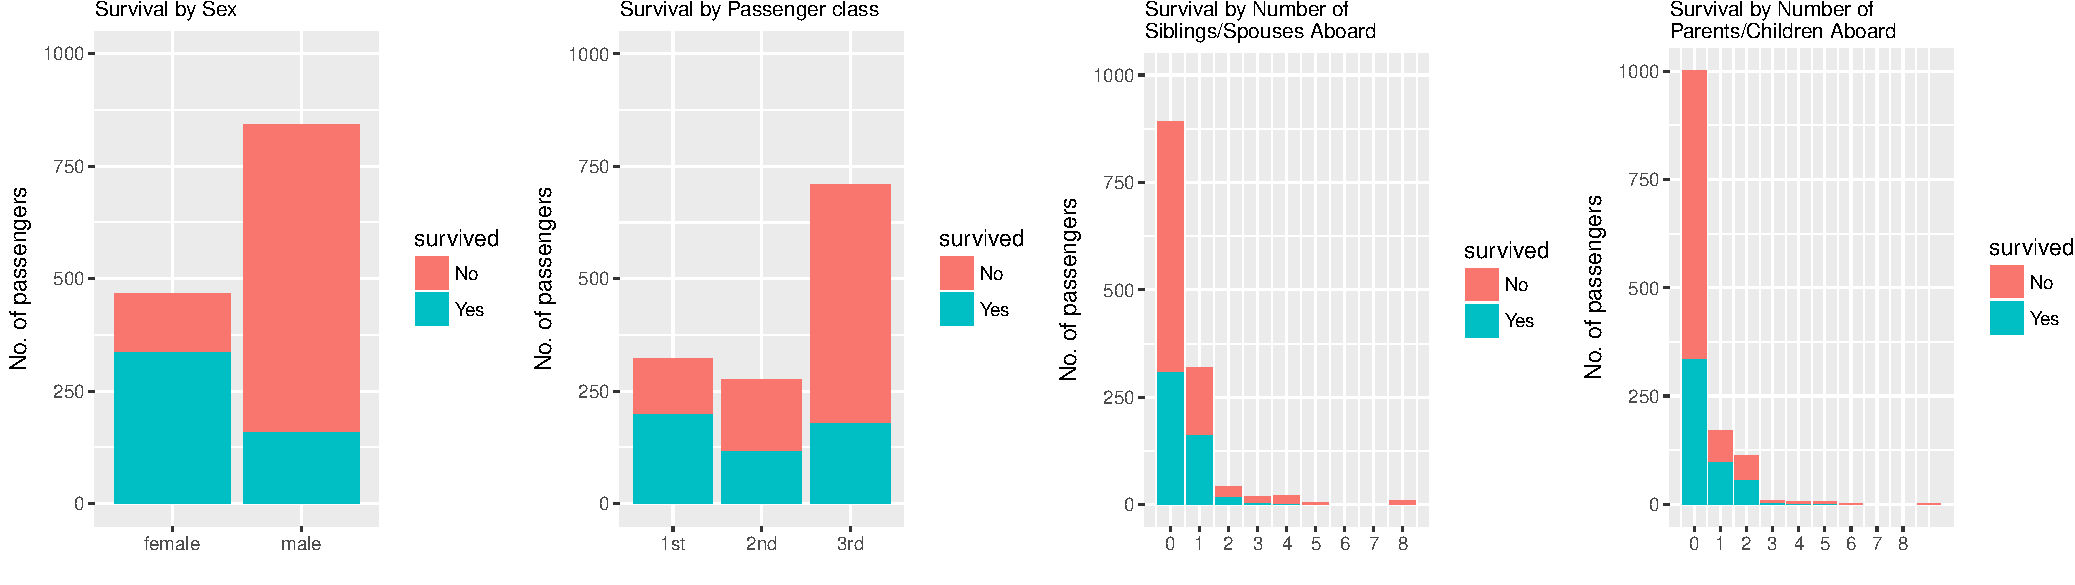
\includegraphics{Seminararbeit_1_Gruppe_2_files/figure-latex/unnamed-chunk-7-1.pdf}

We learn the following things from these bar plots:

\begin{itemize}
\tightlist
\item
  \emph{sex}: Females have a much higher chance of survival than males.
  The \emph{sex} feature is important in our predictions
\item
  \emph{pclass}: Passengers from 3rd class are less likely to survive
  than those from 1st and 2rd class.
\item
  \emph{sibsp} and \emph{parch}: having too many
  siblings/spouses/parents/children on board or travelling alone would
  decrease the chance of surviving. Travelling with one or two family
  members seems to raise the survival chances of the individuals.
\end{itemize}

For metric features \emph{age} and \emph{fare} we use box plots.

\begin{Shaded}
\begin{Highlighting}[]
\NormalTok{p5 <-}\StringTok{ }\KeywordTok{ggplot}\NormalTok{(titanic, }\KeywordTok{aes}\NormalTok{(}\DataTypeTok{y =}\NormalTok{ age, }\DataTypeTok{x =}\NormalTok{ survived, }\DataTypeTok{fill =}\NormalTok{ survived)) }\OperatorTok{+}
\StringTok{    }\KeywordTok{geom_boxplot}\NormalTok{() }\OperatorTok{+}
\StringTok{    }\KeywordTok{labs}\NormalTok{(}\DataTypeTok{subtitle =} \StringTok{"Boxplot age"}\NormalTok{, }\DataTypeTok{y =} \StringTok{"Age"}\NormalTok{, }\DataTypeTok{x =} \StringTok{" "}\NormalTok{)}

\NormalTok{p6 <-}\StringTok{ }\KeywordTok{ggplot}\NormalTok{(titanic, }\KeywordTok{aes}\NormalTok{(}\DataTypeTok{y =}\NormalTok{ fare, }\DataTypeTok{x =}\NormalTok{ survived, }\DataTypeTok{fill =}\NormalTok{ survived)) }\OperatorTok{+}\StringTok{ }
\StringTok{    }\KeywordTok{geom_boxplot}\NormalTok{() }\OperatorTok{+}
\StringTok{    }\KeywordTok{labs}\NormalTok{(}\DataTypeTok{subtitle =} \StringTok{"Boxplot fare"}\NormalTok{, }\DataTypeTok{y =} \StringTok{"Fares"}\NormalTok{, }\DataTypeTok{x =} \StringTok{" "}\NormalTok{) }

\KeywordTok{grid.arrange}\NormalTok{(p5,p6,}\DataTypeTok{ncol =} \DecValTok{2}\NormalTok{)}
\end{Highlighting}
\end{Shaded}

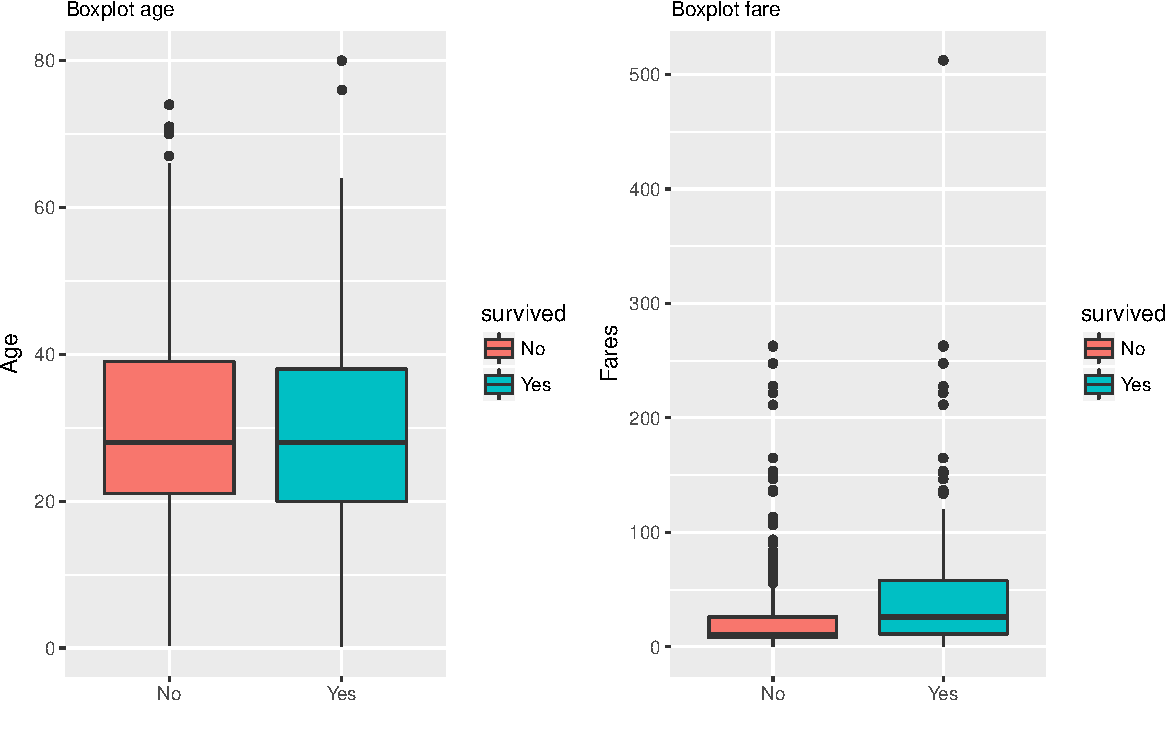
\includegraphics{Seminararbeit_1_Gruppe_2_files/figure-latex/unnamed-chunk-8-1.pdf}

It could be also useful to use a bar plot for metric features to see the
trend better:

\begin{Shaded}
\begin{Highlighting}[]
\NormalTok{p7 <-}\StringTok{ }\KeywordTok{ggplot}\NormalTok{(titanic, }\KeywordTok{aes}\NormalTok{(}\DataTypeTok{x =}\NormalTok{ age, }\DataTypeTok{fill =}\NormalTok{ survived)) }\OperatorTok{+}\StringTok{ }
\StringTok{    }\KeywordTok{geom_histogram}\NormalTok{(}\DataTypeTok{position =} \StringTok{"fill"}\NormalTok{, }\DataTypeTok{bins =} \DecValTok{30}\NormalTok{) }\OperatorTok{+}
\StringTok{    }\KeywordTok{labs}\NormalTok{(}\DataTypeTok{subtitle =} \StringTok{"Survival by age"}\NormalTok{, }\DataTypeTok{y =} \StringTok{"Percentages"}\NormalTok{, }\DataTypeTok{x =} \StringTok{" "}\NormalTok{) }\OperatorTok{+}
\StringTok{    }\KeywordTok{scale_x_continuous}\NormalTok{(}\DataTypeTok{breaks =} \KeywordTok{seq}\NormalTok{(}\DecValTok{0}\NormalTok{, }\DecValTok{90}\NormalTok{, }\DataTypeTok{by =} \DecValTok{10}\NormalTok{))}

\NormalTok{p8 <-}\StringTok{ }\KeywordTok{ggplot}\NormalTok{(titanic, }\KeywordTok{aes}\NormalTok{(}\DataTypeTok{x =}\NormalTok{ fare, }\DataTypeTok{fill =}\NormalTok{ survived)) }\OperatorTok{+}\StringTok{ }
\StringTok{    }\KeywordTok{geom_histogram}\NormalTok{(}\DataTypeTok{position =} \StringTok{"fill"}\NormalTok{, }\DataTypeTok{bins =} \DecValTok{30}\NormalTok{) }\OperatorTok{+}
\StringTok{    }\KeywordTok{labs}\NormalTok{(}\DataTypeTok{subtitle =} \StringTok{"Survival by fare"}\NormalTok{, }
         \DataTypeTok{y =} \StringTok{"Percentages"}\NormalTok{, }\DataTypeTok{x =} \StringTok{" "}\NormalTok{) }

\KeywordTok{grid.arrange}\NormalTok{(p7,p8,}\DataTypeTok{ncol =} \DecValTok{2}\NormalTok{)}
\end{Highlighting}
\end{Shaded}

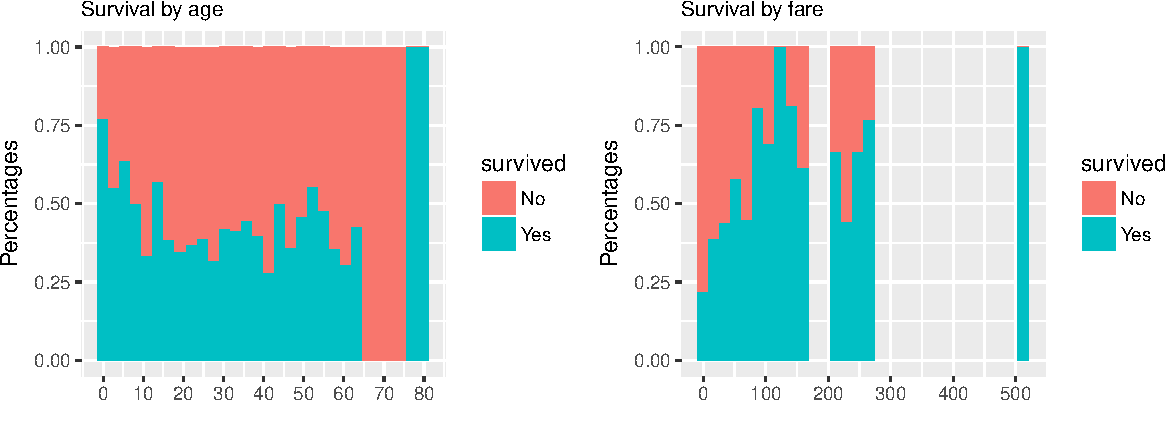
\includegraphics{Seminararbeit_1_Gruppe_2_files/figure-latex/unnamed-chunk-9-1.pdf}

\begin{itemize}
\tightlist
\item
  \emph{fare} and \emph{age} contains some outliers, which should be
  treated later.
\item
  The chance of survival shows a declining tendency, although all oldest
  passengers (about 80 years old) had survived. Passengers from 65-75
  years old have the lowest chance of survival.
\item
  The higher the fare is, the higher is the chance of survival.
\end{itemize}

It could be also helpful to take a look at the relationship of
explanatory features:

\begin{Shaded}
\begin{Highlighting}[]
\NormalTok{dropValue <-}\StringTok{ }\KeywordTok{c}\NormalTok{(}\StringTok{"name"}\NormalTok{,}\StringTok{"cabin"}\NormalTok{,}\StringTok{"ticket"}\NormalTok{,}\StringTok{"boat"}\NormalTok{,}\StringTok{"body"}\NormalTok{,}\StringTok{"home.dest"}\NormalTok{)}
\NormalTok{corDataframe <-}\StringTok{ }\NormalTok{titanic[ , }\OperatorTok{!}\NormalTok{(}\KeywordTok{names}\NormalTok{(titanic) }\OperatorTok\StringTok{ }\NormalTok{dropValue)] }
\NormalTok{corDataframe <-}\StringTok{ }\KeywordTok{sapply}\NormalTok{(corDataframe, }\ControlFlowTok{function}\NormalTok{(x) x <-}\StringTok{ }\KeywordTok{as.integer}\NormalTok{(x))}
\KeywordTok{round}\NormalTok{(}\KeywordTok{cor}\NormalTok{(}\KeywordTok{na.omit}\NormalTok{(corDataframe)), }\DataTypeTok{digits =} \DecValTok{2}\NormalTok{)}
\end{Highlighting}
\end{Shaded}

\begin{verbatim}
##          pclass survived   sex   age sibsp parch  fare embarked
## pclass     1.00    -0.32  0.14 -0.41  0.05  0.02 -0.57     0.28
## survived  -0.32     1.00 -0.54 -0.06 -0.01  0.12  0.25    -0.20
## sex        0.14    -0.54  1.00  0.07 -0.10 -0.22 -0.19     0.11
## age       -0.41    -0.06  0.07  1.00 -0.24 -0.15  0.18    -0.08
## sibsp      0.05    -0.01 -0.10 -0.24  1.00  0.37  0.14     0.05
## parch      0.02     0.12 -0.22 -0.15  0.37  1.00  0.22     0.01
## fare      -0.57     0.25 -0.19  0.18  0.14  0.22  1.00    -0.30
## embarked   0.28    -0.20  0.11 -0.08  0.05  0.01 -0.30     1.00
\end{verbatim}

\begin{itemize}
\tightlist
\item
  Our target feature \emph{survived} correlates mostly to \emph{sex} and
  \emph{pclass}, followed by \emph{fare} and \emph{embarked}.
\item
  \emph{pclass} and \emph{fare} correlates strongly negative to each
  other. So the first class is more expensive than second and third
  class.
\item
  \emph{pclass} also correlates quite strongly with \emph{age}. But it
  could also be a spurious correlation.
\item
  \emph{sibsp} and \emph{parch} also correlate, since both declare
  family size
\end{itemize}

Let us show some multiple relationships graphically:

\begin{Shaded}
\begin{Highlighting}[]
\NormalTok{p9 <-}\StringTok{ }\KeywordTok{ggplot}\NormalTok{(titanic,}\KeywordTok{aes}\NormalTok{(pclass, }\DataTypeTok{fill =}\NormalTok{ survived)) }\OperatorTok{+}\StringTok{ }
\StringTok{    }\KeywordTok{facet_grid}\NormalTok{( }\OperatorTok{~}\StringTok{ }\NormalTok{sex) }\OperatorTok{+}\StringTok{ }
\StringTok{    }\KeywordTok{geom_bar}\NormalTok{() }\OperatorTok{+}\StringTok{ }\KeywordTok{labs}\NormalTok{(}\DataTypeTok{subtitle =} \StringTok{"Survival by sex and passenger class"}\NormalTok{,}
                      \DataTypeTok{y =} \StringTok{"No. of passengers"}\NormalTok{)}

\NormalTok{p10 <-}\StringTok{ }\KeywordTok{ggplot}\NormalTok{(}\KeywordTok{subset}\NormalTok{(titanic, }\OperatorTok{!}\KeywordTok{is.na}\NormalTok{(embarked)), }\KeywordTok{aes}\NormalTok{(}\DataTypeTok{x =}\NormalTok{ pclass, }\DataTypeTok{fill =}\NormalTok{ survived)) }\OperatorTok{+}
\StringTok{    }\KeywordTok{facet_grid}\NormalTok{( }\OperatorTok{~}\StringTok{ }\NormalTok{embarked) }\OperatorTok{+}\StringTok{ }\KeywordTok{geom_bar}\NormalTok{(}\DataTypeTok{position =} \StringTok{"dodge"}\NormalTok{) }\OperatorTok{+}\StringTok{ }
\StringTok{    }\KeywordTok{labs}\NormalTok{(}\DataTypeTok{subtitle =} \StringTok{"Survival by embarked and passenger class"}\NormalTok{, }
         \DataTypeTok{y =} \StringTok{"No. of passengers"}\NormalTok{, }\DataTypeTok{x =} \StringTok{""}\NormalTok{) }\OperatorTok{+}\StringTok{ }\KeywordTok{ylim}\NormalTok{(}\DecValTok{0}\NormalTok{,}\DecValTok{500}\NormalTok{)}

\NormalTok{p11 <-}\StringTok{ }\KeywordTok{ggplot}\NormalTok{(titanic, }\KeywordTok{aes}\NormalTok{(}\DataTypeTok{y =}\NormalTok{ fare, }\DataTypeTok{x =}\NormalTok{ survived, }\DataTypeTok{fill =}\NormalTok{ survived)) }\OperatorTok{+}
\StringTok{    }\KeywordTok{facet_grid}\NormalTok{( }\OperatorTok{~}\StringTok{ }\NormalTok{pclass) }\OperatorTok{+}\StringTok{ }
\StringTok{    }\KeywordTok{geom_boxplot}\NormalTok{() }\OperatorTok{+}\StringTok{ }
\StringTok{    }\KeywordTok{labs}\NormalTok{(}\DataTypeTok{subtitle =} \StringTok{"Survival by fare and passenger class"}\NormalTok{,}
         \DataTypeTok{y =} \StringTok{"Fare"}\NormalTok{) }

\NormalTok{p12 <-}\StringTok{ }\KeywordTok{ggplot}\NormalTok{(titanic, }\KeywordTok{aes}\NormalTok{(}\DataTypeTok{y =}\NormalTok{ age, }\DataTypeTok{x =}\NormalTok{ survived, }\DataTypeTok{fill =}\NormalTok{ survived)) }\OperatorTok{+}
\StringTok{    }\KeywordTok{facet_grid}\NormalTok{( }\OperatorTok{~}\StringTok{ }\NormalTok{pclass) }\OperatorTok{+}\StringTok{ }\KeywordTok{geom_boxplot}\NormalTok{() }\OperatorTok{+}\StringTok{ }
\StringTok{    }\KeywordTok{labs}\NormalTok{(}\DataTypeTok{subtitle =} \StringTok{"Survival by age and passenger class"}\NormalTok{,}
         \DataTypeTok{y =} \StringTok{"Age"}\NormalTok{) }

\KeywordTok{grid.arrange}\NormalTok{(p9, p10, p11, p12, }\DataTypeTok{ncol =} \DecValTok{2}\NormalTok{)}
\end{Highlighting}
\end{Shaded}

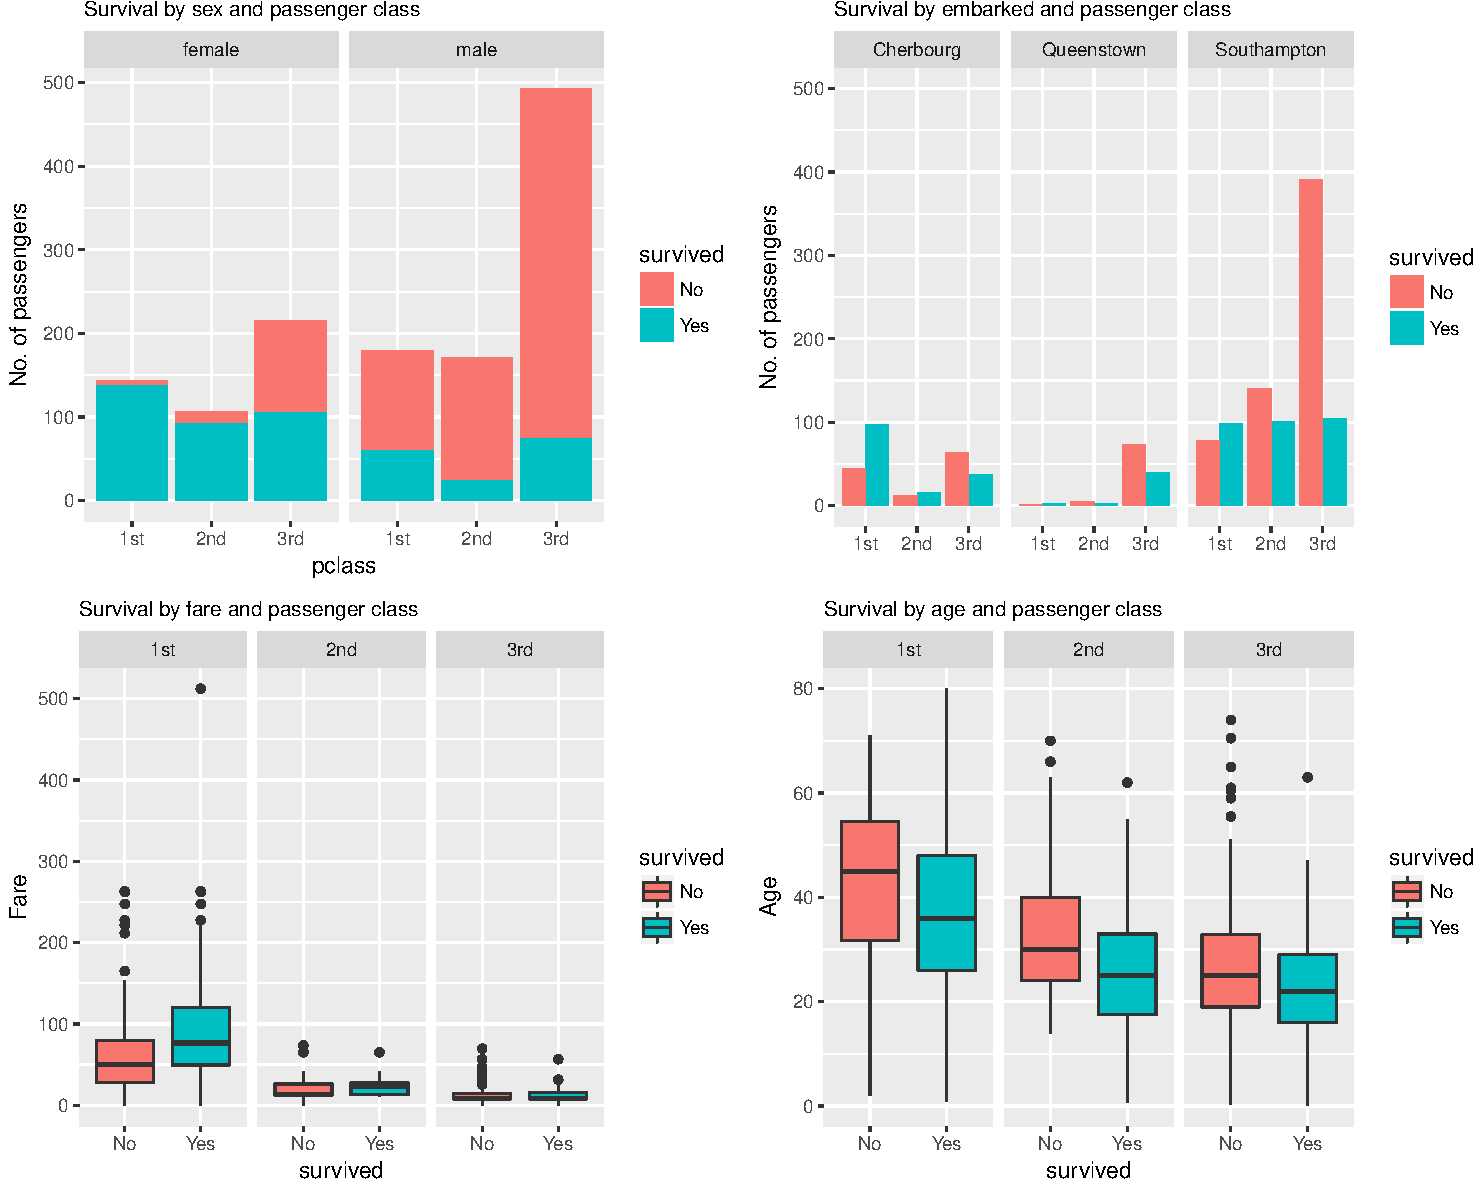
\includegraphics{Seminararbeit_1_Gruppe_2_files/figure-latex/unnamed-chunk-11-1.pdf}

\begin{itemize}
\tightlist
\item
  Female passengers in the first and second class are mostly survived,
  meanwhile men in all classes have a similar chance of survival, which
  is quite low.
\item
  A major of passenger embarked in Southampton. Most of them did not
  survive, especially those in second and third classes.
\item
  Unsurprisingly the first class is the most expensive one. The average
  fare of survived passengers is also higher in the first and second
  classes. This information could be better explained if we have more
  information about the relationship between \emph{pclass} and
  \emph{cabin}.
\item
  The average age of first class passenger (regardless of survival) is
  higher than the rest.
\end{itemize}

That might be enough with plots. Let's move to the next step to choose
the most important features for our model.

\subsection{Identification of relevant
regressors}\label{identification-of-relevant-regressors}

Since some features do not to contain a lot useful information to our
model - or indicates a nearly one to one relationship with the target
feature - we drop them from our model. These are: \emph{name, cabin,
ticket, boat, body, home.dest}

\begin{itemize}
\tightlist
\item
  We assume that the name of a passenger does not have any influence on
  his/her chance of survival. (Although it might be possible to extract
  some useful information from this variable, such as social class. But
  for simplicity purposes, we decided to leave it out of our model)
\item
  We also ignore cabin, since its amount of missing values is too big.
\item
  Apparently the chance of survival does not depend on ticket and
  home-destination. The boat number and body identification number are
  available only after the Titanic had sunk. So they should not be
  involved in the model as well.
\end{itemize}

Let's drop these irrelevant features.

\begin{Shaded}
\begin{Highlighting}[]
\NormalTok{dropValue <-}\StringTok{ }\KeywordTok{c}\NormalTok{(}\StringTok{"name"}\NormalTok{,}\StringTok{"cabin"}\NormalTok{,}\StringTok{"ticket"}\NormalTok{,}\StringTok{"boat"}\NormalTok{,}\StringTok{"body"}\NormalTok{,}\StringTok{"home.dest"}\NormalTok{)}
\NormalTok{titanic <-}\StringTok{  }\NormalTok{titanic[ , }\OperatorTok{!}\NormalTok{(}\KeywordTok{names}\NormalTok{(titanic) }\OperatorTok\StringTok{ }\NormalTok{dropValue)] }

\CommentTok{# source: https://stackoverflow.com/questions/4605206}
\end{Highlighting}
\end{Shaded}

\textbf{Missing values}:\\
In the following segment, we check for the missing values pattern with
help from the library \emph{mice}. The output describes with 1's the
available and with 0's the missing values for each variable in an
aggregated manner. That is, on the leftmost column we obtain the sum of
observations matching the available/missing values of the relative row.
Further, on the last row, we obtain the sum of missing values for the
relevant variable. With that, we can have a good overview not only about
how much data went missing, but also some pattern among missing
observations.

\begin{Shaded}
\begin{Highlighting}[]
\KeywordTok{md.pattern}\NormalTok{(titanic)}
\end{Highlighting}
\end{Shaded}

\begin{verbatim}
##      pclass survived sex sibsp parch fare embarked age    
## 1043      1        1   1     1     1    1        1   1   0
##  263      1        1   1     1     1    1        1   0   1
##    1      1        1   1     1     1    0        1   1   1
##    2      1        1   1     1     1    1        0   1   1
##           0        0   0     0     0    1        2 263 266
\end{verbatim}

From the output, we can see that there are 1306 complete observations
(within the subset data frame created above, since in the full data
frame there are more missing values), one observation where only the
variable \emph{fare} is missing, two observations where \emph{embarked}
is missing and 263 where \emph{age} is missing. Differently to the
\emph{fare} and \emph{embarked} variables, 263 (\textasciitilde{}20\%)
is a significant amount and care is advised when dealing with such a
high proportion of missing data. Even more, since it is very plausible
that the data did not go randomly missing, but a more systematic cause
can be underlying the problem. For instance, it is reasonable that the
observations on the deceased passengers is more likely to go missing
that on those who survived. Nonetheless, dropping those observations
completely and neglecting the remaining information that these data
points would convey, also affecting negatively our model.

Let's see how the variable \emph{age} varies in relation to gender and
class.

\begin{Shaded}
\begin{Highlighting}[]
\KeywordTok{kable}\NormalTok{(}
  \KeywordTok{aggregate}\NormalTok{(titanic[}\KeywordTok{c}\NormalTok{(}\DecValTok{2}\NormalTok{,}\DecValTok{4}\OperatorTok{:}\DecValTok{7}\NormalTok{)],}
          \DataTypeTok{by =} \KeywordTok{list}\NormalTok{(titanic}\OperatorTok{$}\NormalTok{pclass, titanic}\OperatorTok{$}\NormalTok{sex),}
          \DataTypeTok{FUN =}\NormalTok{ mean,}
          \DataTypeTok{na.rm =} \OtherTok{TRUE}\NormalTok{,}
          \DataTypeTok{na.action =}\NormalTok{ na.pass), }
  \DataTypeTok{digits =} \DecValTok{3}
\NormalTok{)}
\end{Highlighting}
\end{Shaded}

\begin{longtable}[]{@{}llrrrrr@{}}
\toprule
Group.1 & Group.2 & survived & age & sibsp & parch & fare\tabularnewline
\midrule
\endhead
1st & female & NA & 37.038 & 0.556 & 0.472 & 109.412\tabularnewline
2nd & female & NA & 27.499 & 0.500 & 0.651 & 23.235\tabularnewline
3rd & female & NA & 22.185 & 0.792 & 0.731 & 15.324\tabularnewline
1st & male & NA & 41.029 & 0.341 & 0.279 & 69.888\tabularnewline
2nd & male & NA & 30.815 & 0.327 & 0.193 & 19.905\tabularnewline
3rd & male & NA & 25.962 & 0.471 & 0.256 & 12.415\tabularnewline
\bottomrule
\end{longtable}

\begin{Shaded}
\begin{Highlighting}[]
\CommentTok{# source: https://stackoverflow.com/questions/16844613}
\end{Highlighting}
\end{Shaded}

Due to the great age variation among male female passengers in different
classes, we replace the \texttt{NA} values conditional on their
respective class and sex. This should perform better than naively using
the \texttt{mean()} or \texttt{median()} values.

\begin{Shaded}
\begin{Highlighting}[]
\NormalTok{titanic[}\KeywordTok{is.na}\NormalTok{(titanic}\OperatorTok{$}\NormalTok{age) }\OperatorTok{&}
\StringTok{        }\NormalTok{titanic}\OperatorTok{$}\NormalTok{pclass }\OperatorTok{==}\StringTok{ "1st"} \OperatorTok{&}
\StringTok{        }\NormalTok{titanic}\OperatorTok{$}\NormalTok{sex }\OperatorTok{==}\StringTok{ "female"}\NormalTok{, }\StringTok{"age"}\NormalTok{] <-}\StringTok{ }\FloatTok{37.03759}

\NormalTok{titanic[}\KeywordTok{is.na}\NormalTok{(titanic}\OperatorTok{$}\NormalTok{age) }\OperatorTok{&}
\StringTok{        }\NormalTok{titanic}\OperatorTok{$}\NormalTok{pclass }\OperatorTok{==}\StringTok{ "2nd"} \OperatorTok{&}
\StringTok{        }\NormalTok{titanic}\OperatorTok{$}\NormalTok{sex }\OperatorTok{==}\StringTok{ "female"}\NormalTok{, }\StringTok{"age"}\NormalTok{] <-}\StringTok{ }\FloatTok{27.49919}

\NormalTok{titanic[}\KeywordTok{is.na}\NormalTok{(titanic}\OperatorTok{$}\NormalTok{age) }\OperatorTok{&}
\StringTok{        }\NormalTok{titanic}\OperatorTok{$}\NormalTok{pclass }\OperatorTok{==}\StringTok{ "3rd"} \OperatorTok{&}
\StringTok{        }\NormalTok{titanic}\OperatorTok{$}\NormalTok{sex }\OperatorTok{==}\StringTok{ "female"}\NormalTok{, }\StringTok{"age"}\NormalTok{] <-}\StringTok{ }\FloatTok{22.18531}

\NormalTok{titanic[}\KeywordTok{is.na}\NormalTok{(titanic}\OperatorTok{$}\NormalTok{age) }\OperatorTok{&}
\StringTok{        }\NormalTok{titanic}\OperatorTok{$}\NormalTok{pclass }\OperatorTok{==}\StringTok{ "1st"} \OperatorTok{&}
\StringTok{        }\NormalTok{titanic}\OperatorTok{$}\NormalTok{sex }\OperatorTok{==}\StringTok{ "male"}\NormalTok{, }\StringTok{"age"}\NormalTok{] <-}\StringTok{ }\FloatTok{41.02925}

\NormalTok{titanic[}\KeywordTok{is.na}\NormalTok{(titanic}\OperatorTok{$}\NormalTok{age) }\OperatorTok{&}
\StringTok{        }\NormalTok{titanic}\OperatorTok{$}\NormalTok{pclass }\OperatorTok{==}\StringTok{ "2nd"} \OperatorTok{&}
\StringTok{        }\NormalTok{titanic}\OperatorTok{$}\NormalTok{sex }\OperatorTok{==}\StringTok{ "male"}\NormalTok{, }\StringTok{"age"}\NormalTok{] <-}\StringTok{ }\FloatTok{30.81540}

\NormalTok{titanic[}\KeywordTok{is.na}\NormalTok{(titanic}\OperatorTok{$}\NormalTok{age) }\OperatorTok{&}
\StringTok{        }\NormalTok{titanic}\OperatorTok{$}\NormalTok{pclass }\OperatorTok{==}\StringTok{ "3rd"} \OperatorTok{&}
\StringTok{        }\NormalTok{titanic}\OperatorTok{$}\NormalTok{sex }\OperatorTok{==}\StringTok{ "male"}\NormalTok{, }\StringTok{"age"}\NormalTok{] <-}\StringTok{ }\FloatTok{25.96227}
\end{Highlighting}
\end{Shaded}

\begin{itemize}
\tightlist
\item
  \textbf{fare}: Replace 1 missing value by the mean \emph{fare} in the
  concerned \emph{pclass}.
\end{itemize}

For the variable \emph{fare}, only the following observation is missing:

\begin{Shaded}
\begin{Highlighting}[]
\NormalTok{titanic[}\KeywordTok{is.na}\NormalTok{(titanic}\OperatorTok{$}\NormalTok{fare), ]}
\end{Highlighting}
\end{Shaded}

\begin{verbatim}
##      pclass survived  sex  age sibsp parch fare    embarked
## 1226    3rd       No male 60.5     0     0   NA Southampton
\end{verbatim}

\begin{Shaded}
\begin{Highlighting}[]
  \CommentTok{# Replace the missing values by the median fare of the third class}
\NormalTok{medianFare <-}\StringTok{ }\KeywordTok{median}\NormalTok{(titanic}\OperatorTok{$}\NormalTok{fare[titanic}\OperatorTok{$}\NormalTok{pclass }\OperatorTok{==}\StringTok{ "3rd"}\NormalTok{], }\DataTypeTok{na.rm =} \OtherTok{TRUE}\NormalTok{)}
\NormalTok{titanic}\OperatorTok{$}\NormalTok{fare[}\KeywordTok{is.na}\NormalTok{(titanic}\OperatorTok{$}\NormalTok{fare)] <-}\StringTok{ }\NormalTok{medianFare}
\end{Highlighting}
\end{Shaded}

\begin{itemize}
\tightlist
\item
  \textbf{embarked}: Replace missing value by the most frequent value.
\end{itemize}

\begin{Shaded}
\begin{Highlighting}[]
\KeywordTok{summary}\NormalTok{(titanic}\OperatorTok{$}\NormalTok{embarked)}
\end{Highlighting}
\end{Shaded}

\begin{verbatim}
##   Cherbourg  Queenstown Southampton        NA's 
##         270         123         914           2
\end{verbatim}

\begin{Shaded}
\begin{Highlighting}[]
\NormalTok{titanic}\OperatorTok{$}\NormalTok{embarked[}\KeywordTok{is.na}\NormalTok{(titanic}\OperatorTok{$}\NormalTok{embarked)] <-}\StringTok{ "Southampton"}
\end{Highlighting}
\end{Shaded}

Let's check once again, whether all missing values are handled.

\begin{Shaded}
\begin{Highlighting}[]
\KeywordTok{any}\NormalTok{(}\KeywordTok{is.na}\NormalTok{(titanic))}
\end{Highlighting}
\end{Shaded}

\begin{verbatim}
## [1] FALSE
\end{verbatim}

So that is enough with cleaning the features. We are going to create the
model in the next step.

\subsection{Fitting a regression
model}\label{fitting-a-regression-model}

Let's create a train and test data set. Now we still have 1309
passengers in total.

\begin{Shaded}
\begin{Highlighting}[]
\KeywordTok{set.seed}\NormalTok{(}\DecValTok{1}\NormalTok{)}
\NormalTok{sampleTitanic <-}\StringTok{ }\NormalTok{titanic[}\KeywordTok{sample}\NormalTok{(}\KeywordTok{nrow}\NormalTok{(titanic), }\DataTypeTok{replace =} \OtherTok{FALSE}\NormalTok{),]}
\KeywordTok{head}\NormalTok{(sampleTitanic, }\DecValTok{10}\NormalTok{)}
\end{Highlighting}
\end{Shaded}

\begin{verbatim}
##      pclass survived    sex      age sibsp parch    fare    embarked
## 348     2nd       No   male 42.00000     0     0 13.0000 Southampton
## 487     2nd       No   male 24.00000     0     0 10.5000 Southampton
## 749     3rd       No   male 34.00000     1     1 14.4000 Southampton
## 1187    3rd       No   male 25.96227     2     0 21.6792   Cherbourg
## 264     1st      Yes female 39.00000     1     0 55.9000 Southampton
## 1172    3rd       No   male 14.50000     8     2 69.5500 Southampton
## 1231    3rd       No female  2.00000     0     1 10.4625 Southampton
## 861     3rd      Yes female 26.00000     0     0  7.9250 Southampton
## 819     3rd      Yes female 16.00000     0     0  7.7333  Queenstown
## 81      1st       No   male 41.02925     0     0 26.5500 Southampton
\end{verbatim}

\begin{Shaded}
\begin{Highlighting}[]
\CommentTok{# separate train and test data}
\NormalTok{train <-}\StringTok{ }\NormalTok{sampleTitanic[}\DecValTok{1}\OperatorTok{:}\DecValTok{1100}\NormalTok{,]}
\NormalTok{test <-}\StringTok{ }\NormalTok{sampleTitanic[}\DecValTok{1101}\OperatorTok{:}\DecValTok{1309}\NormalTok{,] }
\end{Highlighting}
\end{Shaded}

Let's fit the logistic regression. Here we use the backward selection to
keep only relevant regressors. A backward selection removes every
regressor from a model step by step and compare the performance of model
with and without this regressor. The criterion used in this case is the
Akaike Information Criterion (AIC). In general, the AIC rewards a model
with high degree of fit, while including a penalty term for each added
parameter.

\begin{Shaded}
\begin{Highlighting}[]
  \CommentTok{# Training a model with all filtered features. Here we use the training data.}
\NormalTok{modelFull <-}\StringTok{ }\KeywordTok{glm}\NormalTok{(survived }\OperatorTok{~}\NormalTok{., }\DataTypeTok{family =}\NormalTok{ binomial, }\DataTypeTok{data =}\NormalTok{ train) }
  \CommentTok{# Run a backward selection}
\NormalTok{modelAIC <-}\StringTok{ }\KeywordTok{step}\NormalTok{(modelFull, }\DataTypeTok{direction =} \StringTok{"backward"}\NormalTok{)}
\end{Highlighting}
\end{Shaded}

\begin{verbatim}
## Start:  AIC=1023.16
## survived ~ pclass + sex + age + sibsp + parch + fare + embarked
## 
##            Df Deviance    AIC
## - fare      1   1003.3 1021.3
## - parch     1   1003.8 1021.8
## <none>          1003.2 1023.2
## - embarked  2   1013.3 1029.3
## - sibsp     1   1015.8 1033.8
## - age       1   1042.9 1060.9
## - pclass    2   1069.5 1085.5
## - sex       1   1267.7 1285.7
## 
## Step:  AIC=1021.32
## survived ~ pclass + sex + age + sibsp + parch + embarked
## 
##            Df Deviance    AIC
## - parch     1   1003.9 1019.9
## <none>          1003.3 1021.3
## - embarked  2   1014.1 1028.2
## - sibsp     1   1015.8 1031.8
## - age       1   1043.2 1059.2
## - pclass    2   1101.0 1115.0
## - sex       1   1271.4 1287.4
## 
## Step:  AIC=1019.85
## survived ~ pclass + sex + age + sibsp + embarked
## 
##            Df Deviance    AIC
## <none>          1003.9 1019.9
## - embarked  2   1014.6 1026.6
## - sibsp     1   1019.0 1033.0
## - age       1   1043.3 1057.3
## - pclass    2   1101.5 1113.5
## - sex       1   1279.1 1293.1
\end{verbatim}

Based on the AIC, the selected model includes the \emph{pclass, sex,
age, sibsp and embarked} features. We were expecting that \emph{fare}
would remain part of the selected model, based on the plots created
above. In any case, it might be due to the fact that the fare price
highly correlates with the ticket classes. In that sense, the actual
price might not contain much \emph{added} information to the model.
Surprisingly, the city where the passengers embarked remains in the
selected model. We expect that this might be due to some correlation
between the port of embarking and the social status of the passenger,
that is not completely captured in the ticket class varible. For the
subsequent analysis, we use the model selected by the AIC. But, for
comparison purposes, we will discuss and compare the results of the
small model (\emph{modelAIC}) - with the ones for the full model
(\emph{modelFull}) in the section 3.7, when we discuss model accuracy.

\subsection{Discussion of model fit}\label{discussion-of-model-fit}

Let's take a look at the significance of regressors in our model.

\begin{Shaded}
\begin{Highlighting}[]
\KeywordTok{summary}\NormalTok{(modelAIC)}
\end{Highlighting}
\end{Shaded}

\begin{verbatim}
## 
## Call:
## glm(formula = survived ~ pclass + sex + age + sibsp + embarked, 
##     family = binomial, data = train)
## 
## Deviance Residuals: 
##     Min       1Q   Median       3Q      Max  
## -2.5705  -0.6690  -0.4341   0.6571   2.6029  
## 
## Coefficients:
##                      Estimate Std. Error z value Pr(>|z|)    
## (Intercept)          4.369486   0.393924  11.092  < 2e-16 ***
## pclass2nd           -1.081288   0.244310  -4.426 9.61e-06 ***
## pclass3rd           -2.190450   0.239827  -9.133  < 2e-16 ***
## sexmale             -2.566980   0.171936 -14.930  < 2e-16 ***
## age                 -0.043334   0.007186  -6.030 1.64e-09 ***
## sibsp               -0.346029   0.097965  -3.532 0.000412 ***
## embarkedQueenstown  -0.629794   0.328419  -1.918 0.055155 .  
## embarkedSouthampton -0.670480   0.204961  -3.271 0.001071 ** 
## ---
## Signif. codes:  0 '***' 0.001 '**' 0.01 '*' 0.05 '.' 0.1 ' ' 1
## 
## (Dispersion parameter for binomial family taken to be 1)
## 
##     Null deviance: 1459.0  on 1099  degrees of freedom
## Residual deviance: 1003.8  on 1092  degrees of freedom
## AIC: 1019.8
## 
## Number of Fisher Scoring iterations: 5
\end{verbatim}

One way of identifying relevant regressors in via the p-value. The
p-value is the result of a test, which under its Null Hypothesis the
variable coefficient is equal to zero, i.e.~irrelevant to explaining the
predicted variable. A low p-value indicates that a low probability of
gathering such an \emph{extreme} estimated value, given the hypothesis
that the \emph{real} value is actually zero. What ``low'' indeed means
is somewhat arbitrary and depends on the model application. In the
selected model, all variables has a p-value lower than 0.05 and is,
therefore, said to be statistically significant, with exception of
\emph{embarkedQueenstown}, which lies marginally above this cut-off
point.

\begin{Shaded}
\begin{Highlighting}[]
\KeywordTok{anova}\NormalTok{(modelAIC, }\DataTypeTok{test =} \StringTok{"Chisq"}\NormalTok{)}
\end{Highlighting}
\end{Shaded}

\begin{verbatim}
## Analysis of Deviance Table
## 
## Model: binomial, link: logit
## 
## Response: survived
## 
## Terms added sequentially (first to last)
## 
## 
##          Df Deviance Resid. Df Resid. Dev  Pr(>Chi)    
## NULL                      1099     1459.0              
## pclass    2   99.341      1097     1359.6 < 2.2e-16 ***
## sex       1  293.263      1096     1066.4 < 2.2e-16 ***
## age       1   34.842      1095     1031.5 3.576e-09 ***
## sibsp     1   16.940      1094     1014.6 3.859e-05 ***
## embarked  2   10.733      1092     1003.9   0.00467 ** 
## ---
## Signif. codes:  0 '***' 0.001 '**' 0.01 '*' 0.05 '.' 0.1 ' ' 1
\end{verbatim}

The anova() function allows us to see the difference between the null
and residuals deviances. The null deviances is 1497.9, which indicates
the performance of the model with only the intercept based on the
Chi-Square values. The difference between the null deviance and the
residual deviance shows how well the actual model performs against the
null model. Again, feature \emph{sex} performs the best regarding the
significant improvement of the residual deviance, following by
\emph{pclass} and \emph{age}. Other features also reduce the residual
deviance, even though just a bit, and the significance are way worse.

\subsection{Interpreting the model}\label{interpreting-the-model}

The interpretation of the parameters in a logistic regression is not as
straightforward as in a (strictly) linear regression. This is due to the
restriction imposed on the dependent variable, which can only take
values between zero and one. This restriction is observed by
constructing a model\footnote{This model derivation is based on the
  lectures notes and slides from \emph{Statistische Modellierung}, given
  by Prof.~Dr.~Schmid last Fall. Another useful resource was the
  \emph{Lecture Notes on Generalized Linear Models} by by Germán
  Rodríguez. Available on \url{http://data.princeton.edu/wws509/notes/}.
  Accessed on 13.11.2017.}, such as

\begin{equation}
\pi_i = P(Y_i = 1 \mid \beta_0 + \beta_1 x_{i1} + \beta_2 x_{i2} + ... + \beta_k x_{ik}) = F(\eta_i)
\end{equation}

where \(\pi_i\) is the probability of a \emph{desired} event happening,
\(\eta_i = \beta_0 + \beta_1 x_{i1} + \beta_2 x_{i2} + ... + \beta_k x_{ik},\)
and \(F()\) is the logit-function defined as

\begin{equation}
logit(\eta_i) = \frac{exp(\eta_i)}{1 + exp(\eta_i)} = \pi_i.
\end{equation}

With that, one cannot directly interpret the variable coefficients. To
circumvent this problem, one can refer to the \emph{odds} of the
occurrence of an event. This is defined as the probability of the event
occurring against the probability that it does not. Formally,

\begin{equation}
Odds(\pi_i) :=  \frac{P(Y = 1)}{P(Y = 0)} = \frac{P(Y = 1)}{1 - P(Y = 1)} = \frac{\pi_i}{1 - \pi_i}.
\end{equation}

This term is often used in gambling scenarios. That is, if the odds of
winning in a hand of poker is 3 to 1 (i.e.~3/1 or 3:1), it is expected
that the player wins 3 times out of every 4 games, which equals to 75
percent. And, as expected \(3 = \frac{0.75}{1 - 0.75}\).

From Equations (2) and (3), one can show that

\begin{equation}
\frac{\pi_i}{1 - \pi_i} = 
      \frac{\frac{exp(\eta_i)}{1 + exp(\eta_i)} }  {\frac{1}{1 + exp(\eta_i)}} =
      exp(\eta_i).
\end{equation}

Moreover, taking the log on both sides of equation (4), one gets

\begin{equation}
log \left(  \frac{\pi_i}{1 - \pi_i}  \right) = \eta_i = \beta_0 + \beta_1 x_{i1} + \beta_2 x_{i2} + ... + \beta_k x_{ik}. 
\end{equation}

Furthermore, due to the product rule of exponentials, one can show that

\begin{equation}
Odds_1(\pi \mid x_{i1}) = \frac{P(Y = 1 \mid x_{i1})}{P(Y = 0 \mid x_{i1})} = 
              exp(\beta_0) \cdot exp(\beta_1 x_{i1}) \cdot~...~\cdot exp(\beta_k x_{ik}).
\end{equation}

And, if one increases \(x_{i1}\) by one unit, while keeping other
variables constant, one gets

\begin{equation}
Odds_2(\pi \mid x_{i1} + 1) = \frac{P(Y = 1 \mid x_{i1} + 1)}{P(Y = 0 \mid x_{i1} + 1)} = 
              exp(\beta_0) \cdot exp(\beta_1 (x_{i1} + 1)) \cdot~...~\cdot exp(\beta_k x_{ik}). 
\end{equation}

Finally, if we divide \(Odds_2\) by \(Odds_1\), what is defined as the
\emph{Odds Ratio} between the two scenarios, we see that all terms
cancel themselves out, leaving only the term with the added unit, as in

\begin{equation}
Odds~Ratio_{(2, 1)} = \frac {Odds_2(\pi, x_{i1} + 1)} {Odds_1(\pi, x_{i1})} = exp(\beta_1).
\end{equation}

For instance, if \(\beta_1 = 0.3\) and \(x_1\),
\(exp(\beta_1) \approx 1.35\), which means that - for a continuous \(x\)
- the \textbf{odds} (not the probability!) of the event occurring
increases by about 35 percent, that means, it gets multiplied by 1.35,
as \(x\) increases by one unit. One can observe that while the Odds
Ratio remains constant for any \(x\), the probability itself depends on
the base value one starts with. In case \(x_1\) was a dummy variable
(such as \(x_1 = 0\), for male and \(x_1 = 1\) for female) and keeping
the same coefficient as illustrated above, than the odds of the event
occurring is 35 percent higher for a female, when comparing to a male
with, otherwise, same characteristics.

In general, if:

\begin{itemize}
\tightlist
\item
  \(\beta_i > 0 \Rightarrow exp(\beta_i) > 1 \Rightarrow Odds~increases\)
\item
  \(\beta_i < 0 \Rightarrow 0 < exp(\beta_i) < 1 \Rightarrow Odds~decreases\)
\item
  \(\beta_i = 0 \Rightarrow exp(\beta_i) = 1 \Rightarrow Odds~remains~constant\)
\end{itemize}

With that in mind, let's have a look at the each coefficient, its
exponential alongside their 95\% confidence intervals.

\begin{Shaded}
\begin{Highlighting}[]
\KeywordTok{kable}\NormalTok{(}\KeywordTok{data.frame}\NormalTok{(}
  \DataTypeTok{coef =} \KeywordTok{round}\NormalTok{(modelAIC}\OperatorTok{$}\NormalTok{coef, }\DecValTok{2}\NormalTok{),}
  \StringTok{"exp_coef"}\NormalTok{ =}\StringTok{ }\KeywordTok{round}\NormalTok{(}\KeywordTok{exp}\NormalTok{(modelAIC}\OperatorTok{$}\NormalTok{coef),}\DecValTok{2}\NormalTok{),}
  \DataTypeTok{confint_low =} \KeywordTok{round}\NormalTok{(}\KeywordTok{exp}\NormalTok{(}\KeywordTok{confint}\NormalTok{(modelAIC)[}\DecValTok{1}\OperatorTok{:}\DecValTok{8}\NormalTok{]),}\DecValTok{2}\NormalTok{),}
  \DataTypeTok{confint_high =} \KeywordTok{round}\NormalTok{(}\KeywordTok{exp}\NormalTok{(}\KeywordTok{confint}\NormalTok{(modelAIC)[}\DecValTok{9}\OperatorTok{:}\DecValTok{16}\NormalTok{]),}\DecValTok{2}\NormalTok{))}
\NormalTok{)}
\end{Highlighting}
\end{Shaded}

\begin{longtable}[]{@{}lrrrr@{}}
\toprule
& coef & exp\_coef & confint\_low & confint\_high\tabularnewline
\midrule
\endhead
(Intercept) & 4.37 & 79.00 & 37.23 & 174.67\tabularnewline
pclass2nd & -1.08 & 0.34 & 0.21 & 0.55\tabularnewline
pclass3rd & -2.19 & 0.11 & 0.07 & 0.18\tabularnewline
sexmale & -2.57 & 0.08 & 0.05 & 0.11\tabularnewline
age & -0.04 & 0.96 & 0.94 & 0.97\tabularnewline
sibsp & -0.35 & 0.71 & 0.58 & 0.85\tabularnewline
embarkedQueenstown & -0.63 & 0.53 & 0.28 & 1.01\tabularnewline
embarkedSouthampton & -0.67 & 0.51 & 0.34 & 0.76\tabularnewline
\bottomrule
\end{longtable}

From the above table, one can observe that all variables, due to the way
the model was specified, has a negative impact in the probability of
survival. More specifically, the odds of an individual from the 2nd
class surviving - while keeping other variables constant - is about a
third of an \emph{similar} individual in the 1st class. A passenger from
the third class has its odds of survival decreased to about a tenth of
one from the 1st class.

The strongest predictor of survival is the variable \emph{sex}. A male
passenger has his odds of survival diminished to about eight percent of
that of a female passenger. Also an increasing \emph{age} has a negative
effect on the chances of surviving the tragedy, but it is not as strong
as the already mentioned variables. We expected a stronger effect of
age, to be inline with the social rule of providing safety and
protection to women and children first. While this is true with women,
the weak effect of age might be due to the fact that the effect is not
linear throughout ones lifetime. As we could see from the plots
discussed above, children had a higher rate of survival, with younger
adults having actually a lower rate and older adults and elderly have a
quite high rate of survival. This may be due to the fact that the ticket
class is correlated with older passengers, and thus, diminishes the
negative effect of survival of an adult when compared to a child. And
that it is also a social rule to protect the elderly first in such
situations.

Surprisingly, the number of siblings or spouses aboard decreases the
odds of survival quite significantly. We suspect that this is due to
people in the lower classes travelling in bigger families, but further
analysis is required in order to test this hypothesis.

Moreover, when compared to the passengers that embarked in Cherbourg,
those from Queenstown are technically (to the statistical significance
of 95\%) not necessarily negatively affect by the chosen city of
embarkment. Those that embarked in Southampton, however, had their odds
of survival decreased by about half.

\subsection{Model Accuracy}\label{model-accuracy}

Let's see how good our model performs regarding the accuracy and compare
to the full model, as specified above.

\begin{Shaded}
\begin{Highlighting}[]
  \CommentTok{# Predict the test data. The column survived is hidden during the predicting.}
\NormalTok{testPredict <-}\StringTok{ }\KeywordTok{predict}\NormalTok{(modelAIC,}\DataTypeTok{type =} \StringTok{'response'}\NormalTok{, }\DataTypeTok{newdata =}\NormalTok{ test[}\OperatorTok{-}\DecValTok{2}\NormalTok{]) }

  \CommentTok{# Assign the results into 2 categories of survival.}
\NormalTok{survivedPredict <-}\StringTok{ }\KeywordTok{ifelse}\NormalTok{(testPredict }\OperatorTok{>}\StringTok{ }\FloatTok{0.5}\NormalTok{,}\StringTok{"Yes"}\NormalTok{,}\StringTok{"No"}\NormalTok{) }

  \CommentTok{# Create a confusion matrix and print it.}
\NormalTok{confusionMatrix <-}\StringTok{ }\KeywordTok{table}\NormalTok{(test[,}\DecValTok{2}\NormalTok{],survivedPredict) }
\NormalTok{confusionMatrix}
\end{Highlighting}
\end{Shaded}

\begin{verbatim}
##      survivedPredict
##        No Yes
##   No  108  17
##   Yes  22  62
\end{verbatim}

\begin{Shaded}
\begin{Highlighting}[]
  \CommentTok{# Calculate the accuracy and print it.}
\NormalTok{accuracy <-}\StringTok{ }\KeywordTok{mean}\NormalTok{(survivedPredict }\OperatorTok{==}\StringTok{ }\NormalTok{test}\OperatorTok{$}\NormalTok{survived)}\OperatorTok{*}\DecValTok{100}
\KeywordTok{print}\NormalTok{(}\KeywordTok{paste}\NormalTok{(}\StringTok{"The (restricted) model accuracy is"}\NormalTok{, }\KeywordTok{round}\NormalTok{(accuracy,}\DataTypeTok{digits =} \DecValTok{2}\NormalTok{), }\StringTok{"%"}\NormalTok{))}
\end{Highlighting}
\end{Shaded}

\begin{verbatim}
## [1] "The (restricted) model accuracy is 81.34 %"
\end{verbatim}

In order to test if the classification is indeed better than randomly
picking values, we conducted the Press's Q Test, which consist of the
following test equation.

\[ Press's~Q = \frac{(n - (n \cdot G \cdot \alpha))^2}{n \cdot(G - 1)} \sim \chi_{1}^{2} \]

\begin{Shaded}
\begin{Highlighting}[]
\NormalTok{n <-}\StringTok{ }\KeywordTok{length}\NormalTok{(titanic}\OperatorTok{$}\NormalTok{survived)}
\NormalTok{pq <-}\StringTok{ }\NormalTok{(n }\OperatorTok{-}\StringTok{ }\NormalTok{n }\OperatorTok{*}\StringTok{ }\DecValTok{2} \OperatorTok{*}\StringTok{ }\NormalTok{accuracy)}\OperatorTok{^}\DecValTok{2}\OperatorTok{/}\NormalTok{n}
\DecValTok{1} \OperatorTok{-}\StringTok{ }\KeywordTok{pchisq}\NormalTok{(pq,}\DecValTok{1}\NormalTok{)}
\end{Highlighting}
\end{Shaded}

\begin{verbatim}
## [1] 0
\end{verbatim}

As one can see, the test indicates that is extremely improbable that the
model randomly assigned the correct values around 81 percent of the
time. In any case, how does the restricted model compares to the full
one, when only considering their predictive power.

For that, we calculate the predictive accuracy for the full model.

\begin{Shaded}
\begin{Highlighting}[]
  \CommentTok{# Predict the test data. The column survived is hidden during the predicting.}
\NormalTok{testPredict2 <-}\StringTok{ }\KeywordTok{predict}\NormalTok{(modelFull,}\DataTypeTok{type =} \StringTok{'response'}\NormalTok{, }\DataTypeTok{newdata =}\NormalTok{ test[}\OperatorTok{-}\DecValTok{2}\NormalTok{]) }

  \CommentTok{# Assign the results into 2 categories of survival.}
\NormalTok{survivedPredict2 <-}\StringTok{ }\KeywordTok{ifelse}\NormalTok{(testPredict2 }\OperatorTok{>}\StringTok{ }\FloatTok{0.5}\NormalTok{,}\StringTok{"Yes"}\NormalTok{,}\StringTok{"No"}\NormalTok{) }

  \CommentTok{# Create a confusion matrix and print it.}
\NormalTok{confusionMatrix <-}\StringTok{ }\KeywordTok{table}\NormalTok{(test[,}\DecValTok{2}\NormalTok{],survivedPredict2) }
\NormalTok{confusionMatrix}
\end{Highlighting}
\end{Shaded}

\begin{verbatim}
##      survivedPredict2
##        No Yes
##   No  111  14
##   Yes  23  61
\end{verbatim}

\begin{Shaded}
\begin{Highlighting}[]
  \CommentTok{# Calculate the accuracy and print it.}
\NormalTok{accuracy <-}\StringTok{ }\KeywordTok{mean}\NormalTok{(survivedPredict2 }\OperatorTok{==}\StringTok{ }\NormalTok{test}\OperatorTok{$}\NormalTok{survived)}\OperatorTok{*}\DecValTok{100}
\KeywordTok{print}\NormalTok{(}\KeywordTok{paste}\NormalTok{(}\StringTok{"The (full) model accuracy is"}\NormalTok{, }\KeywordTok{round}\NormalTok{(accuracy,}\DataTypeTok{digits =} \DecValTok{2}\NormalTok{), }\StringTok{"%"}\NormalTok{))}
\end{Highlighting}
\end{Shaded}

\begin{verbatim}
## [1] "The (full) model accuracy is 82.3 %"
\end{verbatim}

One can observe that the accuracy of the unrestricted model is slightly
superior to that of the restricted one. This model, although includes
variables that are statistically insignificant performs better, when the
application only concerns better classification accuracy. This
exemplifies that a ``best'' model is not a robust concept, since it
always depends on the application intended for the model.
Econometricians usually aspire to construct models with great
explanatory power for each variable. This points towards more
parsimonious models. If, on the other hand, the intend is to create a
model, where the main objective is to achieve predictions as accurate as
possible - as it is the case in machine learning classifiers, for
instance - it would point us towards a bigger model, including variables
that might be statistically insignificant, but increases prediction
accuracy.

There are still several ways to improve the quality of the data set as
well as the performance of our predicted model. There is a method called
k-fold cross validation, which is used to limit problems like
over-fitting (over-fitting: a model which contains too many explanatory
variables than necessary). This method partitioned randomly the data set
into k equal sized subsets. One of these subsets serves as test data and
the rest (k-1) as training data. The cross-validation repeats k-times
and returns k different results, which could be averaged to one final
result.

So that is. We know that there are still several things need to be
improved in our model. But we hope that we did it in the right direction
and got the right idea of analysing a logistic regression from a given
data set.

Thank you in advance.


\end{document}
